\chapter{Building a Tool with XCore}

\epigraph{Software is like entropy. It is difficult to grasp, weighs nothing, and obeys the second law of thermodynamics; i.e. it always increases.}{Norman Ralph Augustine}

XCore is used for building, in a type safe manaer, analysis tools. Why it is important has been presented in the chapters above. 

In the current chapter we will build an analysis tool which is capable of:
        \begin{enumerate}
                \item computing the cyclomatic complexity of a method
                \item displaying the method in the editor
                \item computing how many calls are done to the function using a call graph.
        \end{enumerate}

\section{Createing the Project}

        Before we start we need to download XCore and install it into Eclipse. The instalation is very easy, simply clone the \href{https://github.com/SAlexandru/XCore}{XCore repository}
or download it directly as a zip from \href{https://github.com/SAlexandru/XCore/archive/master.zip}{here}. After you have downloaded the repository go to the XCore/deploy/plugings folder
and copy ther XCore jar into the Eclipse instalation folder called \textit{dropins}. At the time of writing this document we are at version 1.2.0 and the jar is called \textit{XCore\_1.2.0.jar}. 

        For the scope of this article please create a new Eclipse workspace and import from the XCore repository the \textit{Util/XCoreView} (a.k.a Insider View) project. This is a nice ui we have
build in order to test tools build with XCore.

        Now, in the new workspace, create a Plug-in Project. In this project create a lib folder and copy the jar that you find in \textit{XCore/deploy/lib/XCoreInterface\_<version>.jar}. Current version 
for this jar is 1.1.0. After this we have to add the library to the dependecy path using \textit{Project Properties / Java Build Path / Libraries} as can be seen in figure \ref{fig:addJar}. We
also have to make the jar available at runtime from \textit{MANIFEST.MF/Runtime/Classpath} as can be seen in figure \ref{fig:makeAvailable}. 

       \begin{figure}
             \centering
             \scalebox{0.3}{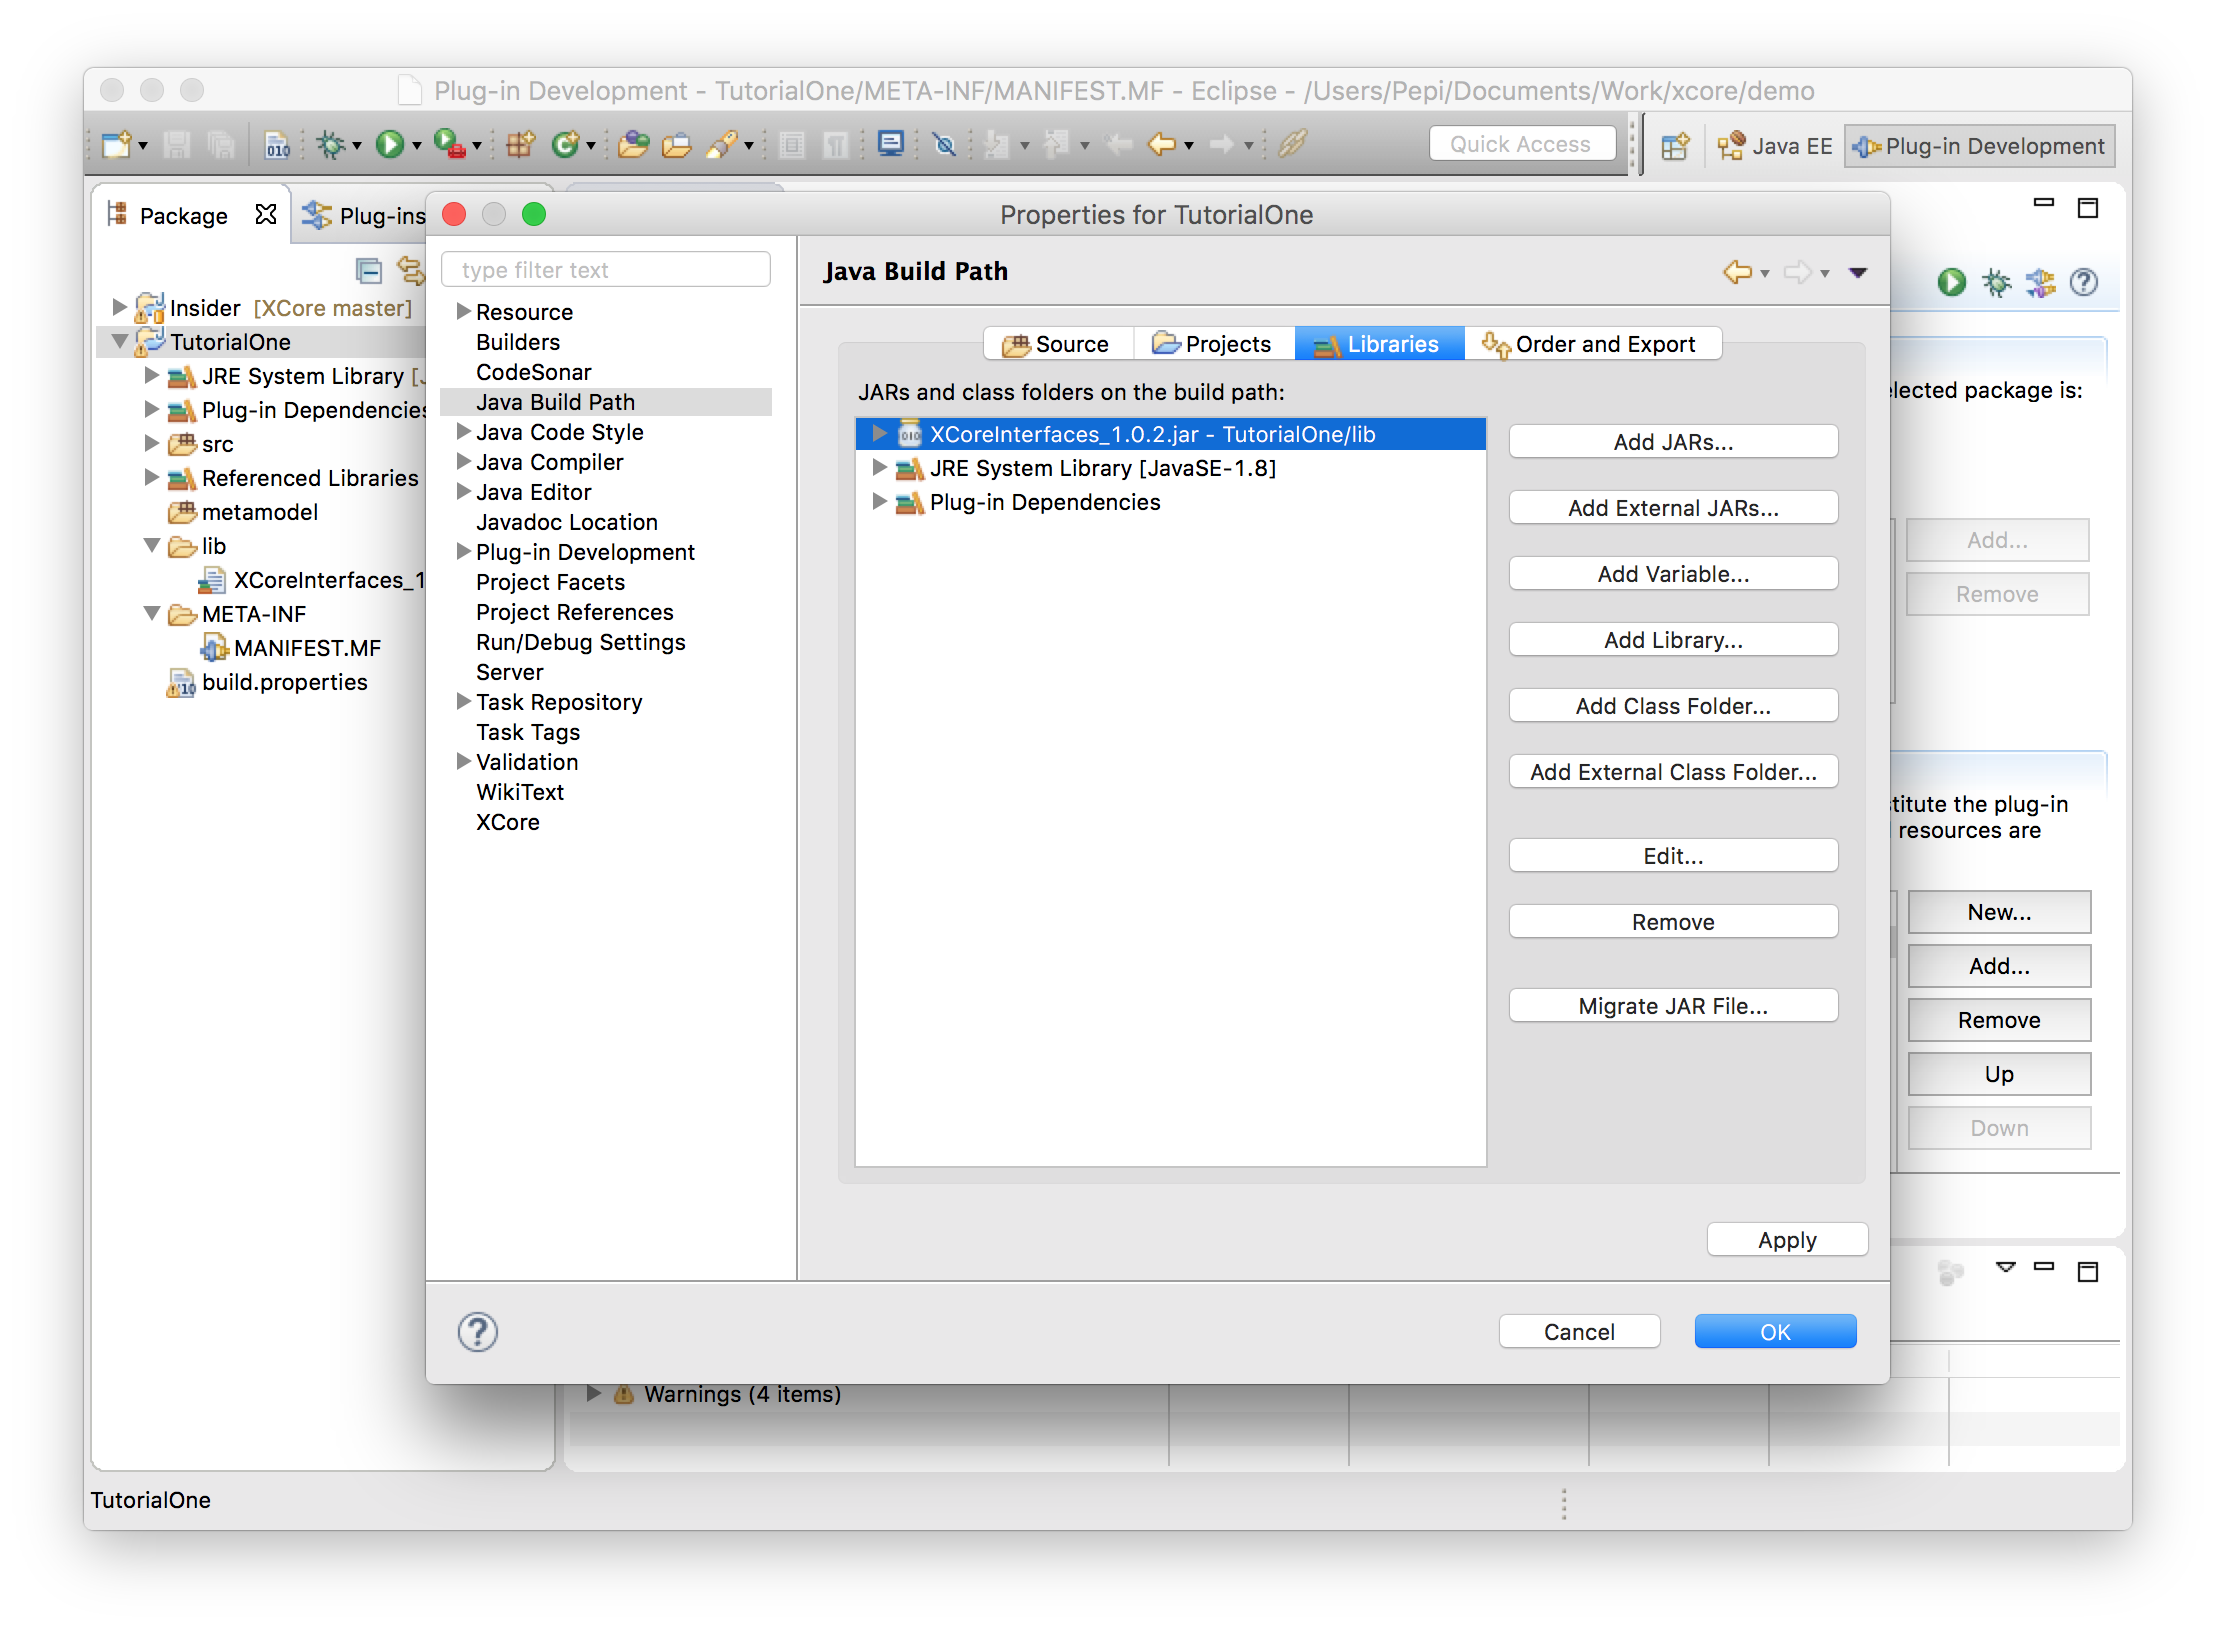
\includegraphics{../img/tutorial/addingJar.png}}
             \caption{Adding the jar to the dependecy}
             \label{fig:addJar}
        \end{figure}    

        \begin{figure}
             \centering
             \scalebox{0.3}{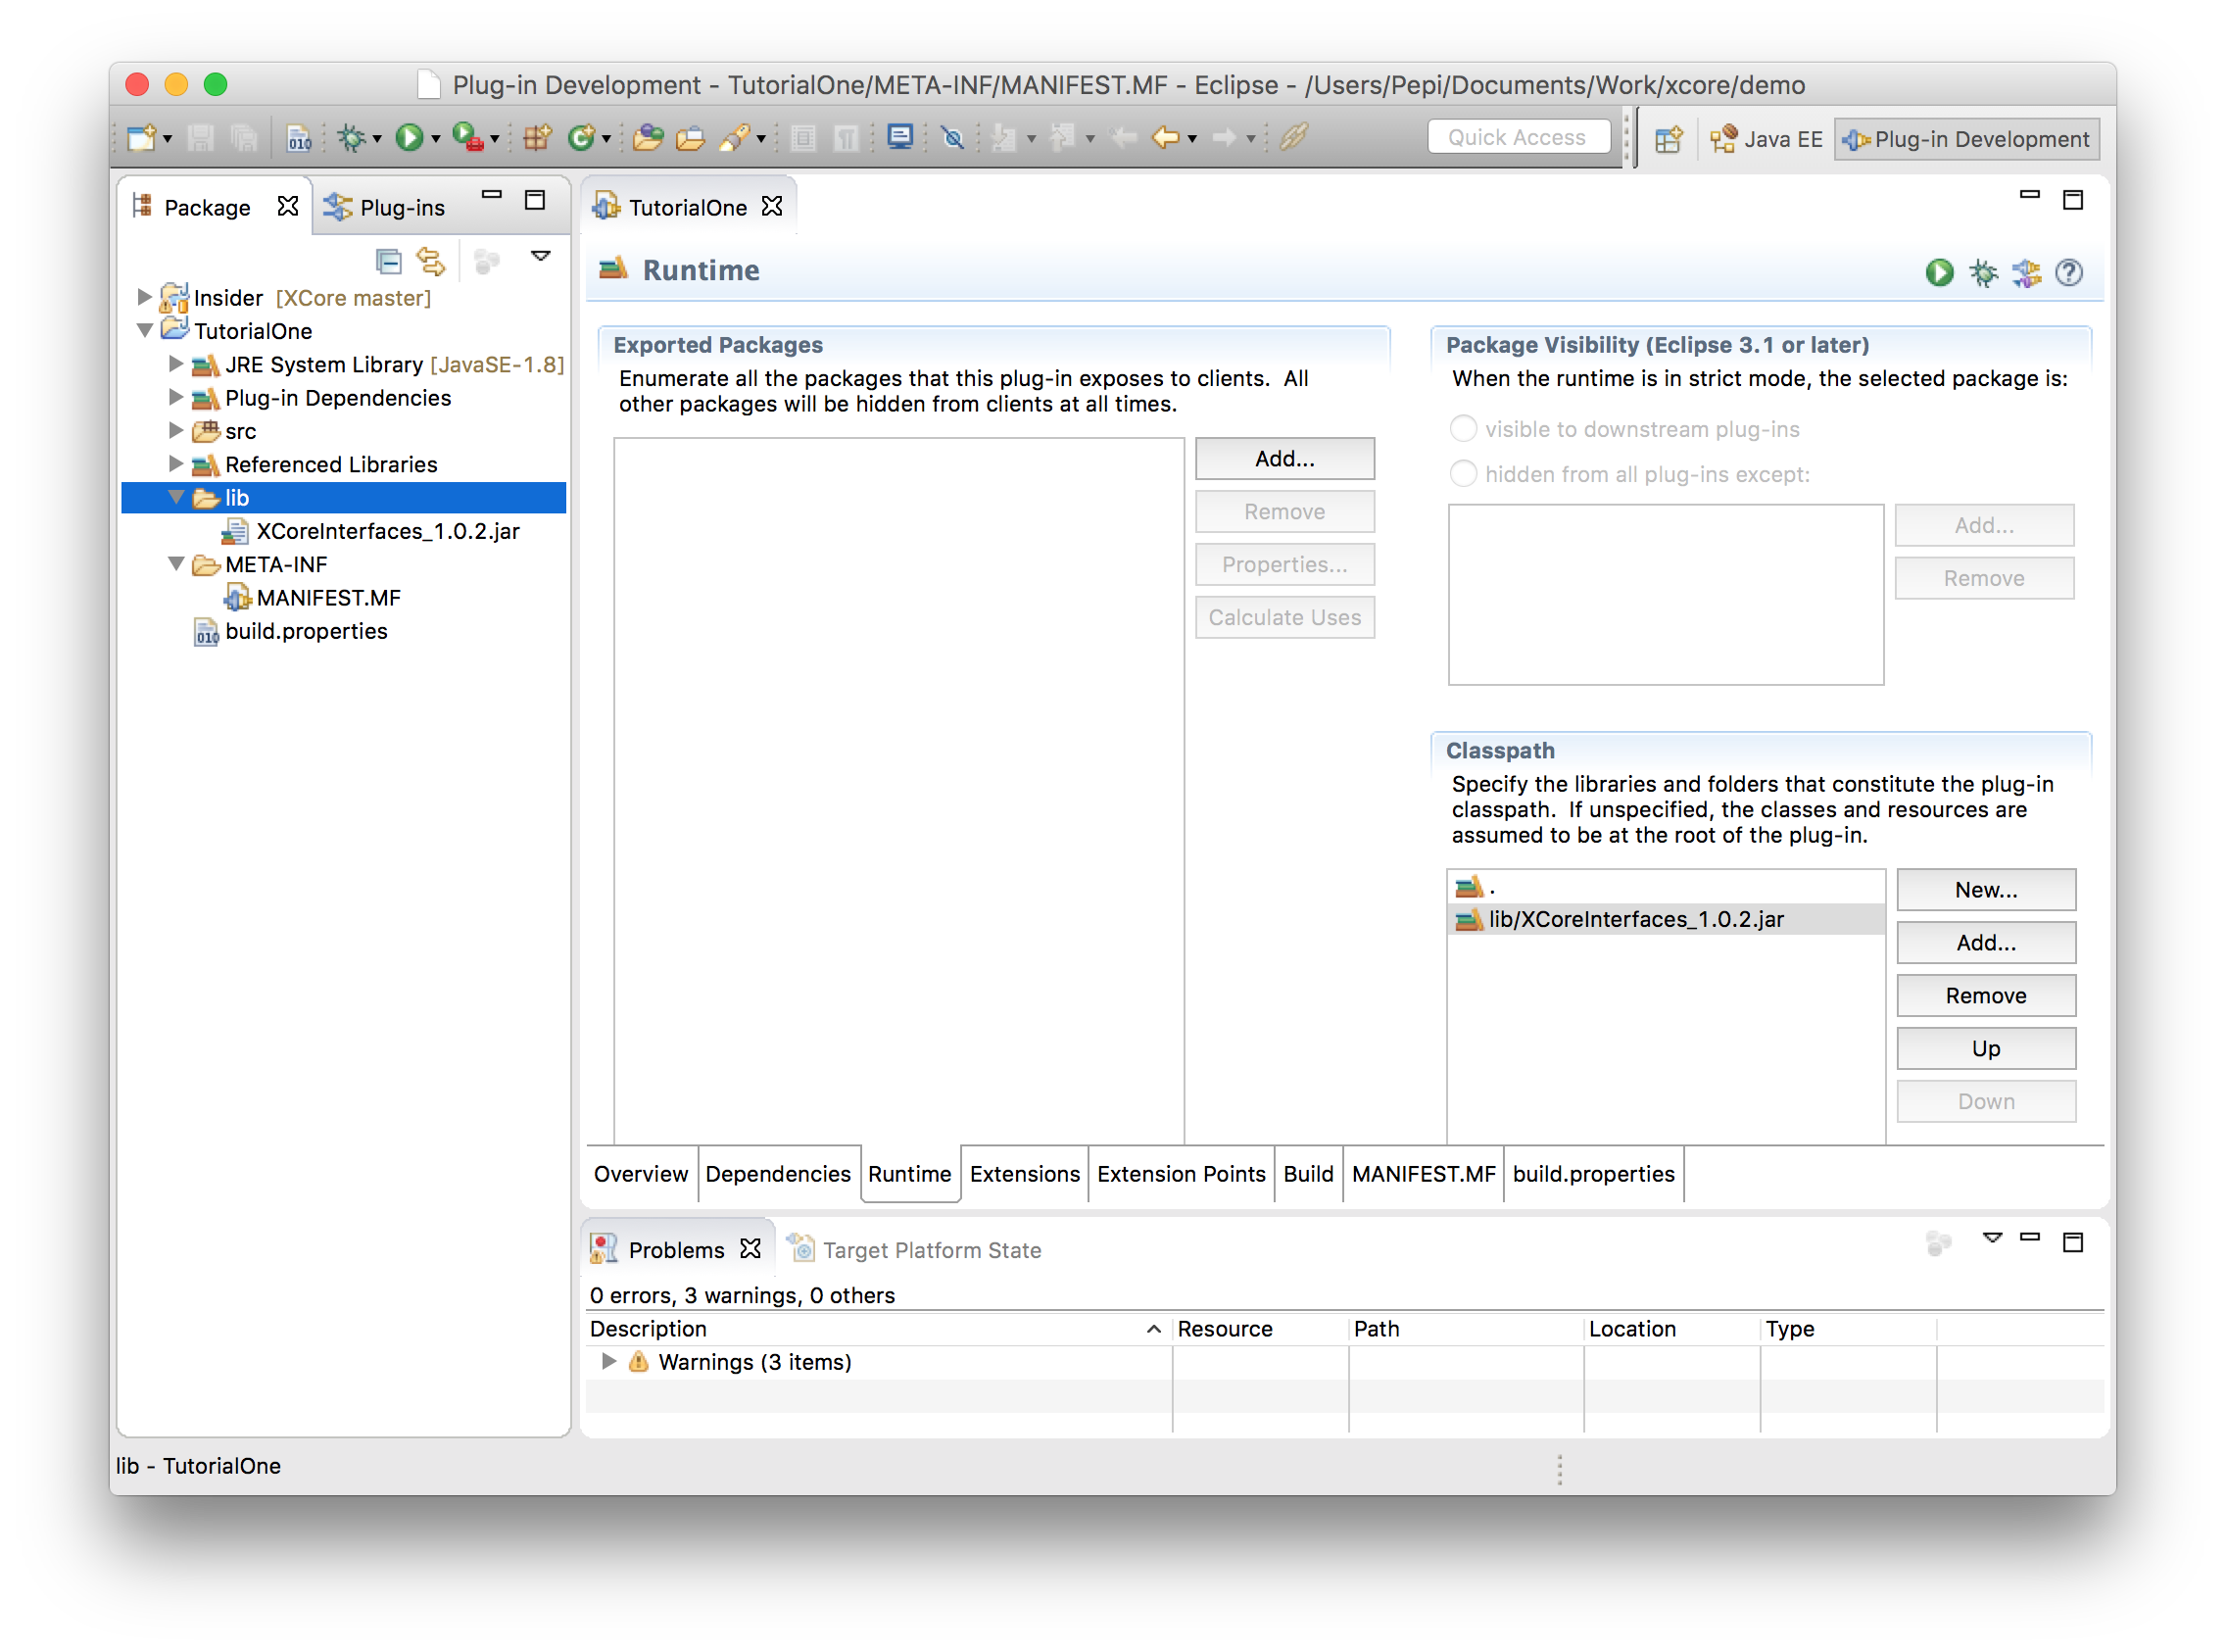
\includegraphics{../img/tutorial/availableAtRuntime.png}}
             \caption{Making the jar available at runtime}
             \label{fig:makeAvailable}
        \end{figure}    


        After this we should enable the annotation processor. This is done by accessing \textit{Project Properties/Java Compiler/Annotation Processing/Factory Path} and ticking the \textit{Enable Specific Settings}.
Also, for clarity we can make the generate content easily accessable by modifing the path from \textit{Project Properties/Java Compiler/Annotation Processing}. Each step is ilustrated in 
figures \ref{fig:enableSpecificSettings} and \ref{fig:modifySourceDir}.

         \begin{figure}
             \centering
             \scalebox{0.3}{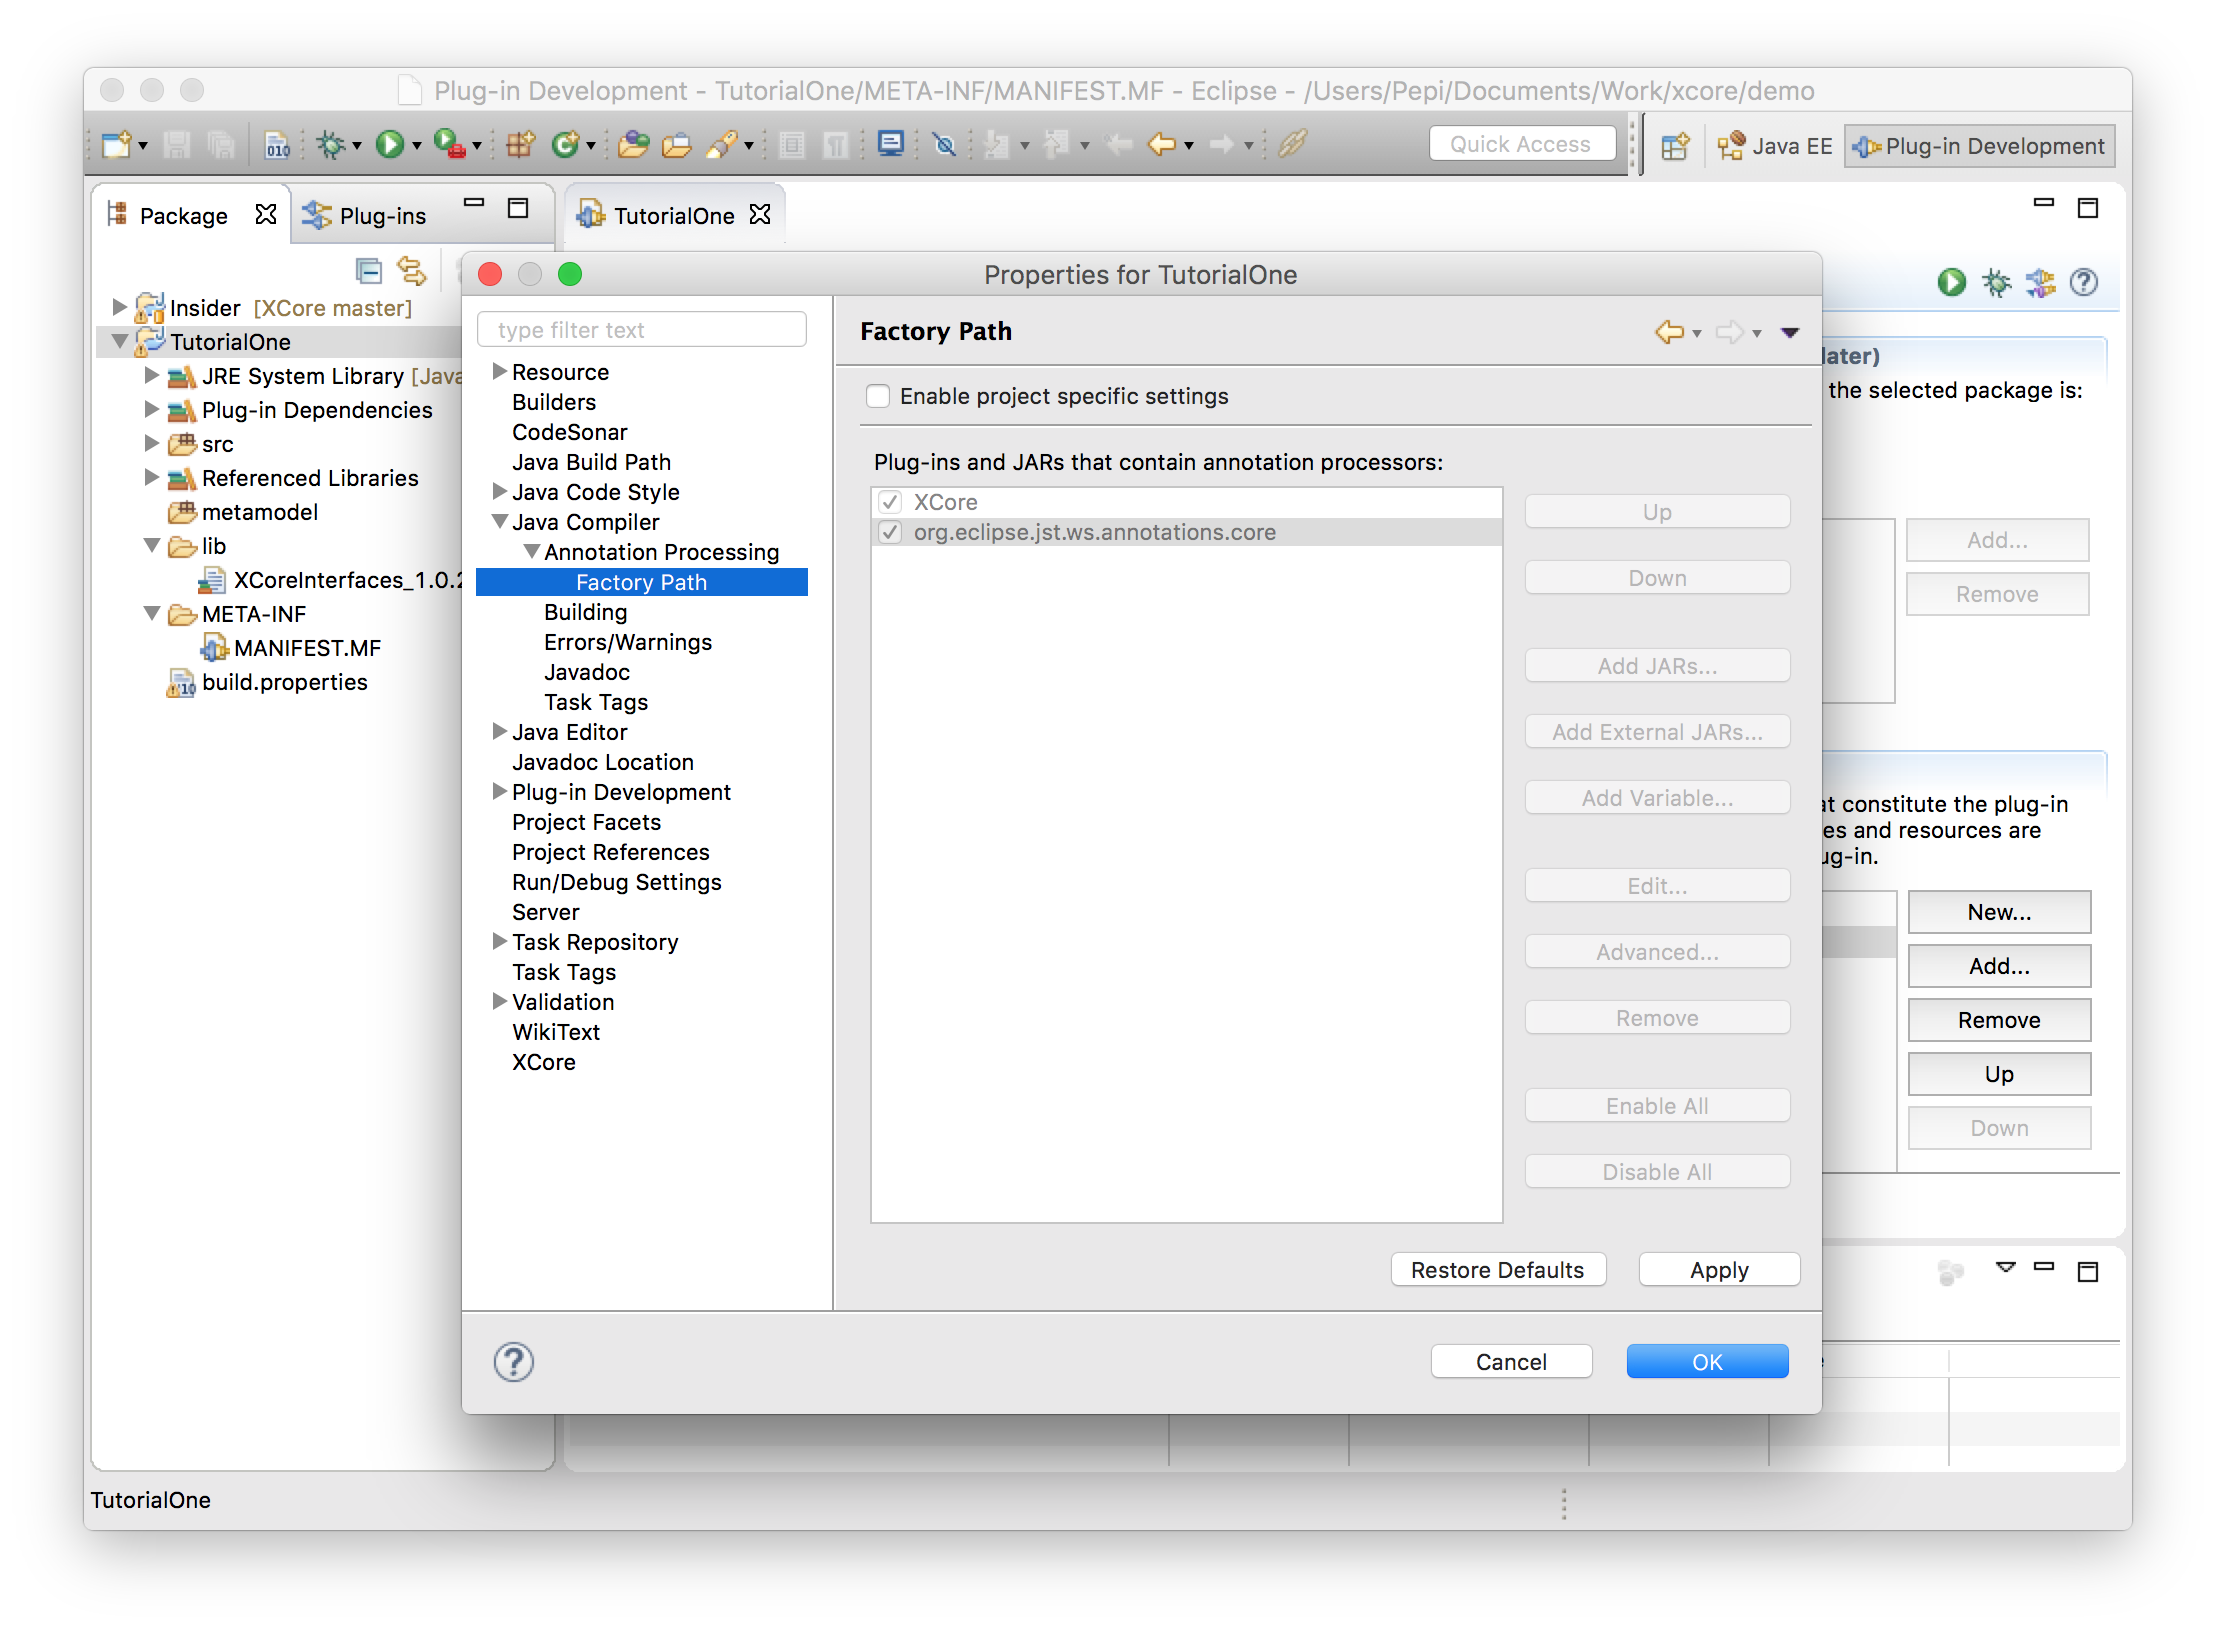
\includegraphics{../img/tutorial/enableXCore.png}}
             \caption{Enable XCore Annotation Processor}
             \label{fig:enableSpecificSettings}
        \end{figure}    

         \begin{figure}
             \centering
             \scalebox{0.3}{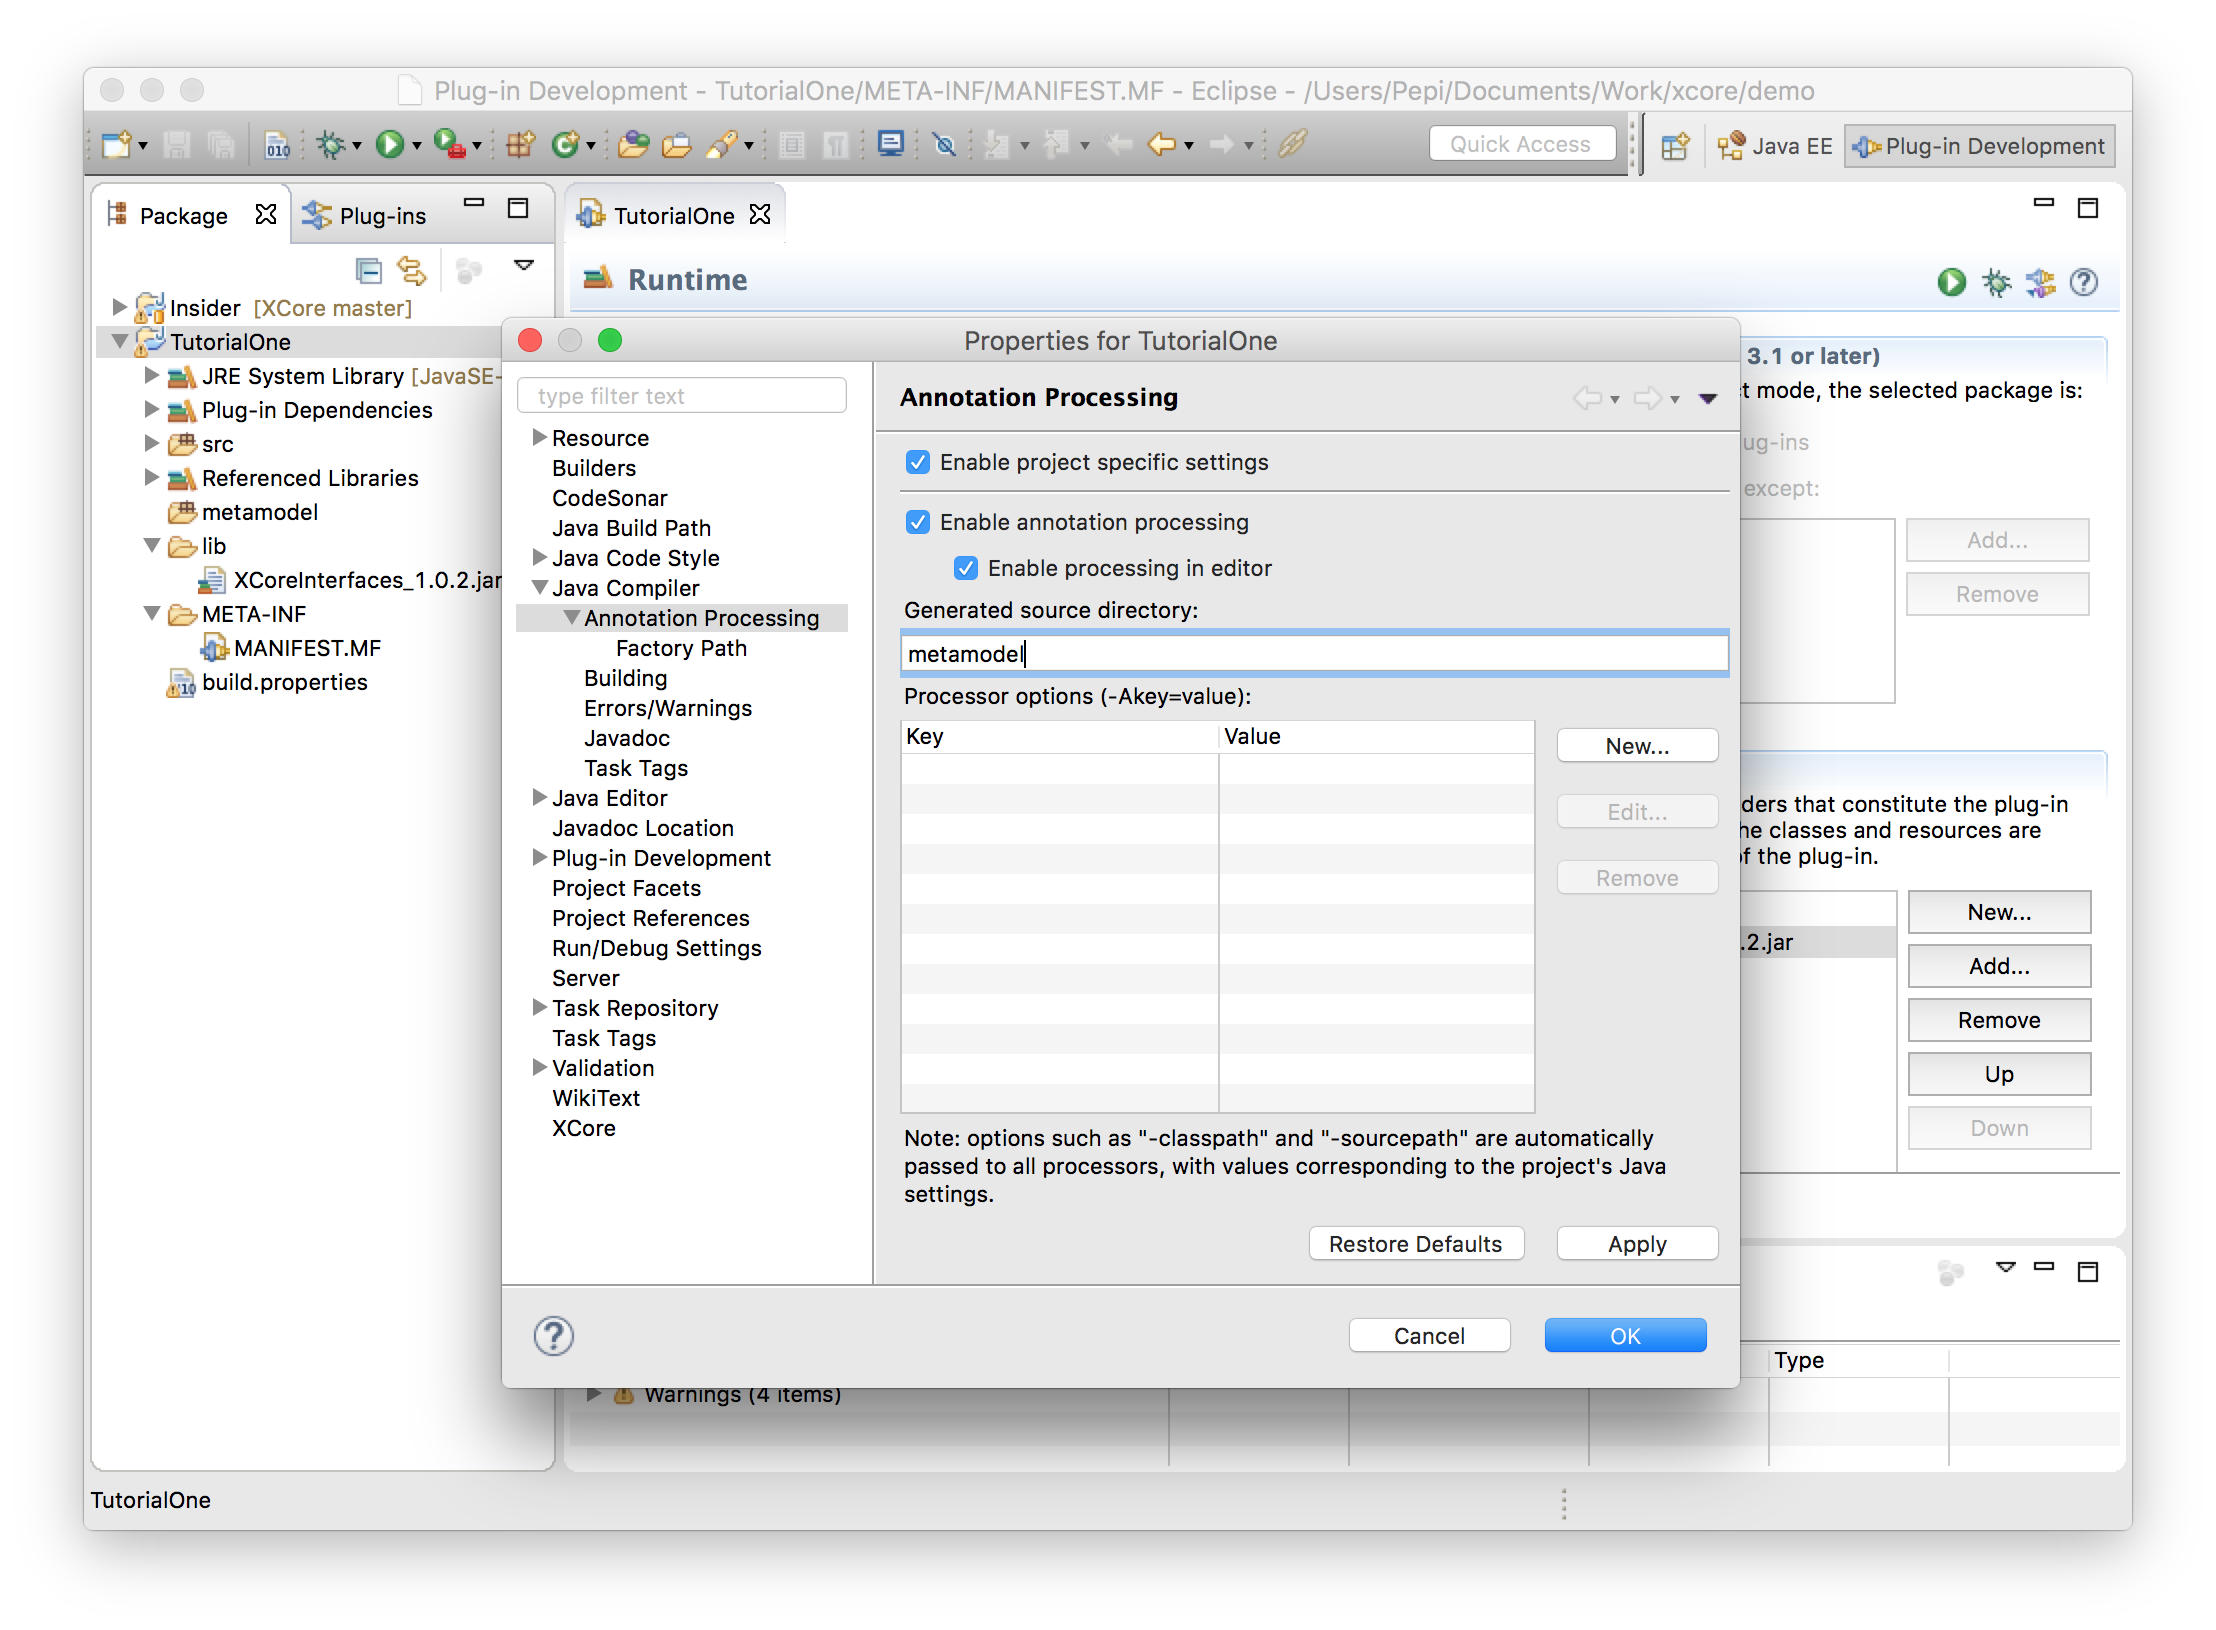
\includegraphics{../img/tutorial/changeSourceDirectory.png}}
             \caption{Change Code Generation Directory}
             \label{fig:modifySourceDir}
        \end{figure}    


\section{Building the Analysises}

        After setting-up the project we continue implementing the analysis mentioned above. We will start implementing the simplest possible tool, which is the displaying the methond in the editor.
        We will also show the new feature that have been developed.

\subsection{Displaying a method in the editor}
       
        First create a class called \code{OpenInEditorAction}. The code for this class is presented in the section \ref{codeSelection:OpenInEditorAction}.
After reading chapter \ref{ch:2} the code should be quite easy to read. We have defined an action class, this can be easily seen by presence of the annotation
\code{@ActionPreformer} and its coressponding interface \code{IActionPerformer<Void, XClass, HListEmpty>}. 
       
        This feature of adding actions on entities has been introduced quite recently into the project. 
        When you first implement this class, you will most likely see that XClass cannot be imported because it doesn't exist yet.  It doesn't exist because we haven run the annotation processor 
which will generate the code for the XClass entity. To invoke the processor, simply build the entire project. Once you have rebuild you can go to the source directory set in the first section of
this chapter and inspect the code. 

        Please note that you should still get a compilation error on the line where you call the methond \code{getUnderlyingObject()}. This is because we haven't associated any back-end to our tool.
For that please se the subsection \ref{subsection:backEnd}

\small
\begin{lstlisting}[language=Java,numbers=left]
import org.eclipse.jdt.core.JavaModelException;
import org.eclipse.jdt.ui.JavaUI;
import org.eclipse.ui.PartInitException;

import com.salexandru.xcore.utils.interfaces.HListEmpty;
import com.salexandru.xcore.utils.interfaces.IActionPerformer;
import com.salexandru.xcore.utils.metaAnnotation.ActionPerformer;

import exampletool.metamodel.entity.XClass;

@ActionPerformer
public class OpenInEditorAction implements IActionPerformer<Void, XClass, HListEmpty> {

 @Override
 public Void performAction(XClass entity, HListEmpty args) {
 try {
    JavaUI.openInEditor(entity.getUnderlyingObject(), true, true);
 } catch (Exception e) {
    e.printStackTrace();
 }
return null;
}

}
\end{lstlisting}
\normalsize{}\label{codeSelection:OpenInEditorAction}

\subsection{Cyclomatic Complexity}

        In this section we will continue to enrich our small analysis tool by adding a simple metric which is applied onto methods. \\
        A property, as explained in the sections above, is nothing more that an analysis / processing that returns a value. The value isn't restricted to any
specific type, it can be anything! \\
        The metric that we will try to build is called the \textit{Cyclomatic Complexity} of a method. It requires us to compute the number of different paths
that can be executed within the method. Take for example the method presented in \ref{codeSelection:cycloEg}. The cyclomatic complexity is 3. We have one path
then goes through the \textit{then} branch, one that goes through the \textit{else} branch and doesn't enter the while loop and one that goes through the \textit{else}
branch and enters the while loop. 

\small
\begin{lstlisting}[language=Java,numbers=left]
 int method (int x) {
    if (x % 2) return 1;
    else {
        while (x % 2 == 0) x /= 2;
        return x;
    }
 }
\end{lstlisting}
\normalsize{}\label{codeSelection:cycloEg}

        The code for implementing it cyclomatic complexity property can be found below in \ref{codeSelection:cyclomaticComplexity}.
It should be quite strait forward to read. We take the AST of a the methond in question and for each statement: \code{if}, \code{else}
\code{case}, \code{default}, \code{for}, \code{while}, \code{do \{\} while}, \code{try}, \code{catch}, \code{finally} we increase the 
cyclomatic complexity.

\small
\begin{lstlisting}[language=Java, numbers=left]
@PropertyComputer
public class CyclomaticComplexity implements IPropertyComputer<Integer, XMethod> {
@Override
public Integer compute(XMethod entity) {
ASTParser astParser = ASTParser.newParser(AST.JLS8);

astParser.setSource(entity.getUnderlyingObject().getCompilationUnit());


NodeVisitor visitor = new NodeVisitor(entity.toString());
astParser.createAST(null).accept(visitor);

return visitor.getCount();
}

private static final class NodeVisitor extends ASTVisitor {
private int count = 0;
private final String methodName;

public NodeVisitor(final String methodName) {
    this.methodName = methodName;
}

@Override
public boolean visit(MethodDeclaration d) {
    return d.getName().toString().equals(methodName);
}

@Override
public boolean visit(IfStatement node) {
    ++count;
    if (null != node.getElseStatement()) {
        ++count;
    }
    return true;
}

@Override
public boolean visit(ForStatement node) {
    ++count;
    return true;
}

@Override
public boolean visit(SwitchCase node) {
    ++count;
    return true;
}

@Override
public boolean visit(ConditionalExpression node) {
    ++count;
    if (null != node.getElseExpression()) {
        ++count;
    }
    return true;
}

@Override
public boolean visit(InfixExpression node) {
    InfixExpression.Operator type = node.getOperator();
    
    if (InfixExpression.Operator.CONDITIONAL_AND == type ||
        InfixExpression.Operator.CONDITIONAL_OR == type) {
        ++count;
    }
    
    return true;
}

@Override
public boolean visit(WhileStatement node) {
    ++count;
    return true;
}

@Override
public boolean visit(DoStatement node) {
    ++count;
    return true;
}

@Override
public boolean visit(CatchClause node) {
    ++count;
    return true;
}

@Override
public boolean visit(ThrowStatement node) {
    ++count;
    return true;
}

@Override
public boolean visit(BreakStatement node) {
    ++count;
    return true;
}

@Override
public boolean visit(ContinueStatement node) {
    ++count;
    return true;
}
    
public int getCount() {return count + 1;}	
}
}
\end{lstlisting}
\normalsize{}\label{codeSelection:cyclomaticComplexity}

\subsection{Associate A Backend}\label{subsection:backEnd}
        
        Currently we have implemented a property and an action. Both shouldn't compile as we have not associated any back-end.
As mentioned in the previous chapters XCore is dealing with high-level entities, we do not provide a back-end for extracting the entities from the source
code. But we do provide a way of integrated the tools you build with a real back-end. 
        
        To do this, simply go to \textit{Project Properties/XCore} and you will see a table just like in figure \ref{fig:xcoreTable} , just look at the first one for now ! Select 
XMethod hit the edit button. You should see a search bar where you should be able to write the corresponding the entity name from JDT, it's \textit{IMethod}, see figure \ref{fig:IMethod} and hit enter. Do the
same thing for XClass and the table should look like \ref{fig:xcoreTableFull}. Now if you recompile everything it should compile.

        What we have done here is associated every meta-model entity with an corresponding entity from the Eclipse JDT back-end. This will help us greatly in implementing more analysis tools. Of course, we 
are not restricted to mapping them directly to a JDT entity, you could have provided your own implementation of the \textit{IMethod} if you wished.

        \begin{figure}
             \centering
             \scalebox{0.3}{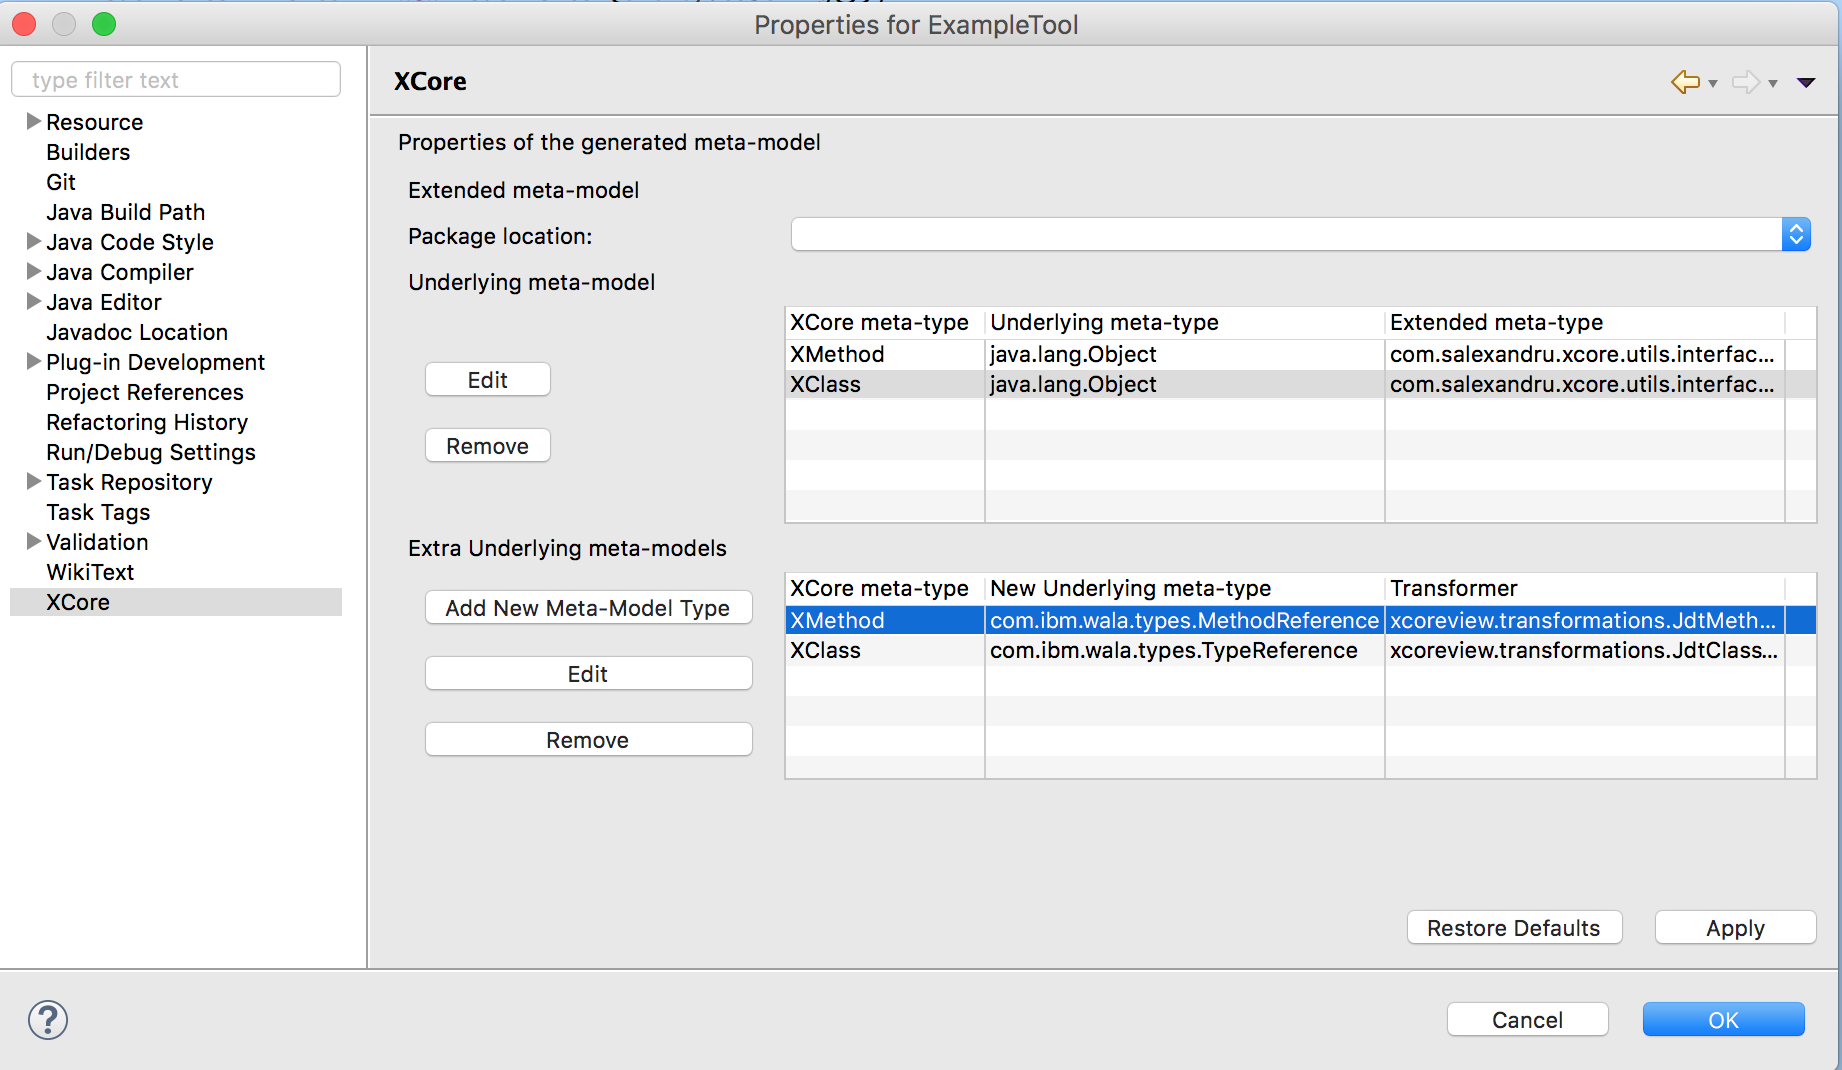
\includegraphics{../img/tutorial/xcoreTable.png}}
             \caption{XCore Project Configuration}
             \label{fig:xcoreTable}
        \end{figure}    

        \begin{figure}
             \centering
             \scalebox{0.3}{\includegraphics{../img/tutorial/iMethond.png}}
             \caption{XCore Search Type Widget}
             \label{fig:IMethond}
        \end{figure}    

        \begin{figure}
             \centering
             \scalebox{0.3}{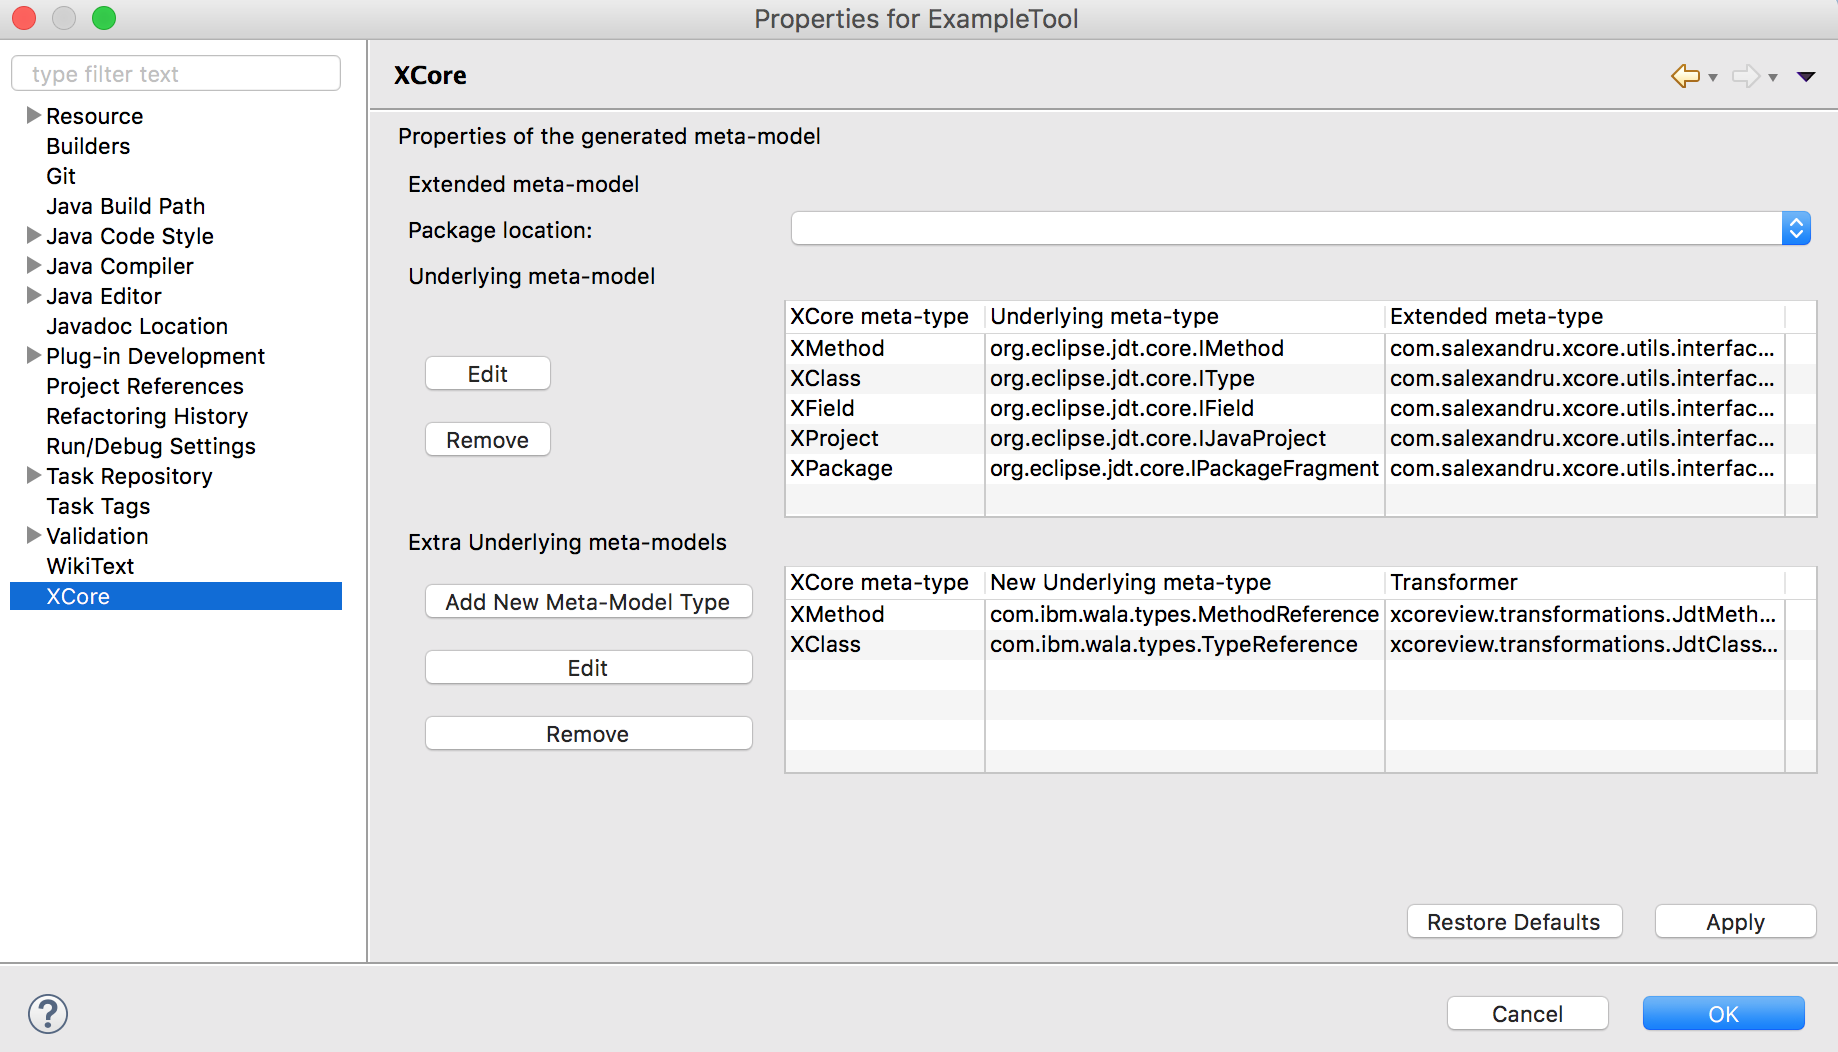
\includegraphics{../img/tutorial/xcoreTableFull.png}}
             \caption{XCore Project Configuration}
             \label{fig:xcoreTableFull}
        \end{figure}    


       

\subsection{Number of calls to the method}

\subsection{Even more}
